%!TEX root = ../template.tex
%%%%%%%%%%%%%%%%%%%%%%%%%%%%%%%%%%%%%%%%%%%%%%%%%%%%%%%%%%%%%%%%%%%%
%% chapter5.tex
%% NOVA thesis document file
%%
%% Chapter with a short latex tutorial and examples
%%%%%%%%%%%%%%%%%%%%%%%%%%%%%%%%%%%%%%%%%%%%%%%%%%%%%%%%%%%%%%%%%%%%

\typeout{NT FILE chapter5.tex}%

\chapter{Ethereum}\label{cha:ethereum}

This chapter provides a detailed description of the Ethereum protocol, 
focusing on its transition from Proof of Work (PoW) to Proof of Stake (PoS) consensus mechanism. 
It also discusses a specific vulnerability known as the bouncing attack, along with a proposed solution and its critical analysis. 
Finally, the chapter outlines the implementation of these concepts in the Mobs simulator, 
including specifications, implementation details, validation processes, and results analysis.
Ethereum has been widely used and provides the foundation of numerous applications, such as non-fungible tokens (NFTs), decentralized finance (DeFi) platforms, and other decentralized apps (dApps).

\section{Protocol Description}\label{sub:protocol_description}

Ethereum is a decentralized blockchain platform that makes smart contract development and execution possible.
Vitalik Buterin made the proposal in 2013, began development in the beginning of 2014 and the network was live on July 30, 2015.
It was intended to be a more adaptable and programmable substitute for Bitcoin, enabling programmers to build decentralized
applications on its platform and use Ether (\textit{ETH}), its native cryptocurrency, to reward network users for processing transactions.

Ethereum, in contrast to Bitcoin, was created as a programmable blockchain platform, enabling programmers to implement logic using Solidity-written smart contracts.
Computational prices are measured via a gas mechanism to guard against resource exhaustion threats and infinite loops.

Ethereum's development has been mainly guided through Ethereum Improvement Proposals (EIPs), community-driven ideas and contributions.

\subsection{PoW to PoS}\label{sub:pow_to_pos}

Ethereum firstly used a Proof of Work (PoW) consensus mechanism, where miners competed to solve complex mathematical problems
in order to validate transactions and generate new blocks, similar to Bitcoin.
Although due to issues with scalability and high energy consumption Ethereum transitioned to a Proof of Stake (PoS) mechanism though an update
referred as The Merge, that started in December 2020 and finished in September 2022.
Validators are now chosen to generate new blocks in PoS based on the amount of ETH they possess and are willing to "stake" as collateral.
This modification improved scalability, security, and energy efficiency, while also reducing energy consumption by over 99\%.
Ethereum's transition to PoS has been successful; however, it has also rendered it susceptible to specific attacks, particularly those that target liveness.
We will now describe one of these attacks along with the solution proposed and implemented by the Ethereum community.

\section{Bouncing attack}\label{sub:bouncing_attack}

Liveness in a blockchain protocol is defined as the ability to always finalize new blocks. These blocks in the
Ethereum protocol are finalized through a process called Casper FFG (Friendly Finality Gadget), in combination with
the LMD GHOST (Latest Message Driven Greediest Heaviest Observed SubTree) fork choice rule.

The Bouncing Attack is an attack that prevents the chain from being finalized by making the main chain
selected in the fork choice rule continually bounce between two candidate chains. The attack leverages the fact that
candidate chains should start from the justified checkpoint with the highest epoch, and Byzantine nodes exploit this by
dividing honest validators opinions, justifying a new checkpoint after some honest validators already have cast their vote.

Justification is the first step in the finalization of a block and a jusfiable checkpoint is a checkpoint that can be justified.
The finalization process is always applied to a checkpoint and a checkpoint neeeds to be justified before being finalized.

The attack becomes possible once there is a justifiable checkpoint in a different branch than the one selected by the fork choice rule it has a
higher epoch than the checkpoint of the branch selected in the fork choice rule. When this happens, Byzantine nodes can now
make honest validators start voting on a different checkpoint in a different chain and thus making the honest validators
bounce their choice between two chains, preventing finalization.


\subsection{Proposed Solution}\label{sub:proposed_patch}

The proposed and implmented solution by the ethereum community to mitigate this attack is simple, add an extra restriction
and prevent validators from changing their mind regarding justified checkpoints after the epoch has passed. This aims to prevent
honest validators from leaving a justifiable checkpoint behind. And even though the seems like a good solution it has a problem,
if byzantine nodes wait long enough to send their messages, those messages can be considered invalid for some honest validators and
just in time by others, thus splitting the votes of honest validators between two chains and not finalizing the checkpoint. This
makes the solution probabilistic and while it may be better and prevent some attacks from malicious actors, it does not completely
protect the network, or guarantees liveness.


\section{Implementation In Mobs}\label{sub:implementation_in_mobs}

To make this implementation in MOBS we followed the specifications in ~\cite{ethereum_analysis} where the attack and 
the finalization process are described in detail. Our goal with this implementation is to check if MOBS can simulate
the protocol, the attack and the proposed solution and has enough information in the locks to detect when the attack happens and
if the solution was effective.

\subsection{Implementation details}\label{sub:implementation_details}

Our implementation focused on fork choice rule and the block finalization, so there were some assumptions we made
to simplify the logic and avoid complexity in parts of the implementation that are not relevant to the attack and the patch:
\begin{itemize}
    \item We assume that the network is consistent throughout the execution of the protocol, meaning no node crash faults
or enters the network after the protocol starts.
    \item We assume that the proposer nodes are the same throughout the execution of the protocol and ignore the random election
described in the Ethereum under scrutiny paper ~\cite{ethereum_under_scrutiny}.
    \item Since it is always not relevant to the attack we assume there will be no Byzantine behaviour regarding message
tampering or message dropping.
\end{itemize}

To achieve this implementation we implemented the following events:

\begin{itemize}
    \item \textbf{Main:} This is the main event in the execution loop and is executed once per slot, a slot is the standard execution time unit and
    there are 32 slots in an epoch. When this event is triggered proposers propose a new block and all nodes attest to justify the epoch's checkpoint,
    A node can attest 3 times per epoch starting from the 11th slot, as defined in the paper.
    \item \textbf{Propose:} This event is triggered when a proposer sends their Propose message and when receiving this message a node simply updates their tree
    and adds the proposed block.
    \item \textbf{Attestation:} When a node sends an attestation message, the receiving node updates their attestation quorum, a hash table where the key is
    the epoch and the value is a list of attestations, only the most recent attestation for each node is kept
    \item \textbf{JustificationFinalization:} In the last slot of each epoch this event is triggered and to simplify and avoid issues with message delays only
    one node justifies and tries to finalyze blocks. First it checks what justifiable checkpoint got the mosst votes this epoch and finalyzes it if the number
    of votes is greater than 2/3 of the total number of nodes. Then it checks the last four justified checkpoints and checks if any of them can be finalized,
    \item \textbf{FinalizedNode:} If a node can be finalized this event is triggered, this acts as a control point for the validation script to know when and which block
    was finalized and when a node receives this message it updates its tree to contain the finalized block.
    \item \textbf{IncrementSlot:} This is a periodic event whose sole purpose is to increment the slot and epoch counter.
\end{itemize}

The implemantation also haas the logic for the attack and the patch. For the attack we have a variable for each node that is set to true
if the execution is Byzantine and false otherwise. In a Byzantine execution a proposer sends a delayed message so that after the attesters
voted we change the checkpoint for the current epoch and preventing the node from finalizing any block, thus making honest nodes bounce between
two nodes belonging to different chains.

For the patch we added a simple check and ignore all proposes after a certain point in the epoch, this ensures that honest nodes do not change their mind
by not being able to attest after receiving a new proposed block.


\subsection{Validation}\label{sub:validation}

To validate the execution of the protocol we created a validation script that checks if for every epoch a block was finalized.
The script reads the log file generated by MOBS and checks which block was finalized in each epoch, if no block was finalized
for more than 5 epochs in a row it sends an error message warning the user.
The tests were executed with 10 nodes, 1 of them was Byzantine and the rest honest.

\begin{figure}[h]
	\centering
	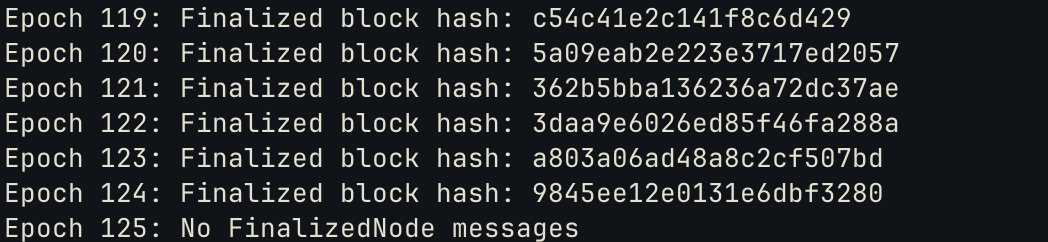
\includegraphics[width=4.5in, angle =0]{ethereum_correct_execution}
	\caption{Output from the log analyser script for an Ethereum correct execution}
	\label{fig:ethereum_correct_execution}
\end{figure}

\begin{figure}[h]
	\centering
	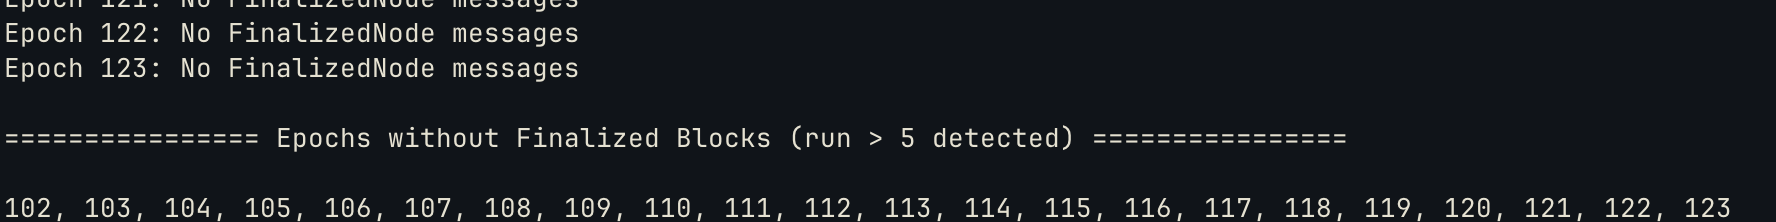
\includegraphics[width=4.5in, angle =0]{ethereum_incorrect_execution}
	\caption{Output from the log analyser script for an Ethereum incorrect execution}
	\label{fig:ethereum_incorrect_execution}
\end{figure}

\subsection{Results analysis}\label{sub:result_analysis}

The results of the validation script were as expected, we were able to detect when the attack happened and that the patch was effective,
just as shown in the figures ~\ref{fig:ethereum_correct_execution} and ~\ref{fig:ethereum_incorrect_execution} above. With more time we would have liked to
do a more detailed analysis and extract more data from the logs, such as the number of votes per checkpoint per epoch, the number of times
the honest nodes bounced between two chains, and the number of times a block was proposed but not finalized.
We would also have liked to do a more thorough test of the patch and try to simulate what is said in the paper~\cite{ethereum_analysis} that
the patch is only a probablistic solution and that if Byzantine nodes waits and sends a message in the correct slote can still split the votes of honest nodes
and keep prevent finalization, but we were not able to do this due to time constraints.